\documentclass[12pt,a4paper]{article}
\usepackage[ngerman]{babel}
\usepackage[utf8]{inputenc}
\usepackage{hyperref}
\usepackage{xcolor}
\usepackage{graphicx}

\title{ORES Custom Documentation II}
%\author{Tom Gülenman}
\date{}
\begin{document}
\maketitle
\textit{Disclaimer: No guarantee for the correctness of information / explanations / sources is given.}
\section{Basic API Usage}
\begin{itemize}
\item \url{http://ores.wmflabs.org/v3/scores/enwiki/?models=draftquality|wp10&revids=34854345|485104318}
\begin{description}
\item Scoring, Context = enwiki, Models (2), RevIDs (2)
\end{description}
\end{itemize}
\section{\href{https://ores.wikimedia.org/v3/\#/}{ORES Scoring Documentation}}
\textit{\url{https://ores.wikimedia.org/v3/\#/}}
\begin{itemize}
\item \href{https://ores.wikimedia.org/v3/scores}{https://ores.wikimedia.org/v3/\colorbox{green}{scores}}
\begin{description}
\item Lists all available contexts (wikis) for scoring
\item 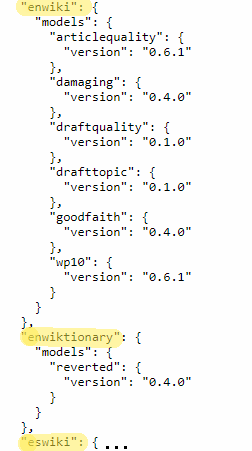
\includegraphics[scale=0.5]{resources/2/ORESscores}
\item Models: reverted, damaging, goodfaith, articlequality, draftquality, drafttopic, wp10, pagelevel, itemquality
\end{description}
\item \href{https://ores.wikimedia.org/v3/scores/enwiki}{https://ores.wikimedia.org/v3/\colorbox{green}{scores}/\colorbox{orange}{\{context\}}}
\begin{description}
\item For example \colorbox{orange}{enwiki}
\item Shows the specified context only
\end{description}
\item \href{https://ores.wikimedia.org/v3/scores/enwiki/870259881}{https://ores.wikimedia.org/v3/\colorbox{green}{scores}/\colorbox{orange}{\{context\}}/\colorbox{cyan}{\{revid\}}}
\begin{description}
\item Shows all scoring information on an edit of the specified context
\item Find revision ID of any article: top right: View history \(\rightarrow\) click on time/data-link \(\rightarrow\) ID displayed in URL at the end
\item 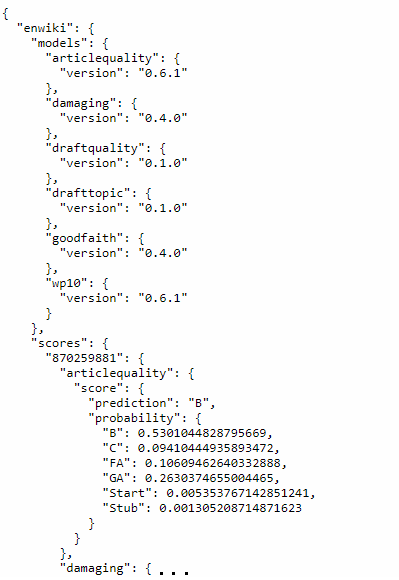
\includegraphics[scale=0.7]{resources/2/ORESscoresId}
\end{description}
\item \href{https://ores.wikimedia.org/v3/scores/enwiki/870259881}{https://ores.wikimedia.org/v3/\colorbox{green}{scores}/\colorbox{orange}{\{context\}}/\colorbox{cyan}{\{revid\}}}/\colorbox{yellow}{\{model\}}
\begin{description}
\item Furthermore a model can be specified
\end{description}
\item Add \href{https://ores.wikimedia.org/v3/scores/?model_info=type}{/?model\_info=\{\colorbox{pink}{model\_info}\}} to any query (at the end!)
\begin{description}
\item For example: \colorbox{pink}{\textit{model\_info}} = \colorbox{green}{type}, \colorbox{green}{statistics}
\item 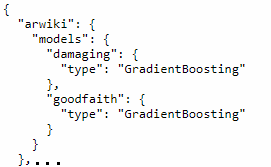
\includegraphics[scale=0.8]{resources/2/ORESscoresType}
\end{description}
\end{itemize}
\section{Specifying parameters}
\begin{itemize}
\item From the paper: \url{https://ores.wikimedia.org/v3/scores/enwiki/?models=damaging&model_info=statistics.thresholds.true.'maximum filter_rate @ recall >= 0.75'}
\begin{description}
\item (spaces: maximum filter\_rate @ recall $>$= 0.75')
\end{description}
\begin{description}
\item Information:
\end{description}
\begin{itemize}
\item only \textbf{damaging}-model
\item model\_info: \textbf{statistics} $\leftarrow$ this is what we need for parameters in our \textit{Visualisierung des Systemverhaltens}
\end{itemize}
\end{itemize}
\section{Parameters}
\subsection{Model: Damaging}
\subsubsection{Thresholds}
Interesting: model\_info=statistics.thresholds.true
\begin{description}
\item Show all true values of parameters (that are not in red below) with the threshold value from 0.002 to 0.987 (not every step, but many!)
\item Without ``.true'' $\rightarrow$ we got double the results divided in false: [...] and true: [...]
\end{description}
\subsubsection{Different parameters}
\begin{itemize}
\item !f1
\item !precision
\item !recall
\item accuracy
\item \textcolor{red}{counts}
\item f1
\item filter\_rate
\item fpr
\item match\_rate
\item \textcolor{red}{pr\_auc}
\item precision
\item \textcolor{red}{rates}
\item recall
\item \textcolor{red}{roc\_auc}
\end{itemize}
\subsection{Model: Articlequality}
\subsubsection{Thresholds}
Interesting: model\_info=statistics.thresholds\\
$\rightarrow$``.true'' doesn't work
\begin{description}
\item Lists for each article quality (Stub to FA) the values for each parameter, given a threshold
\item 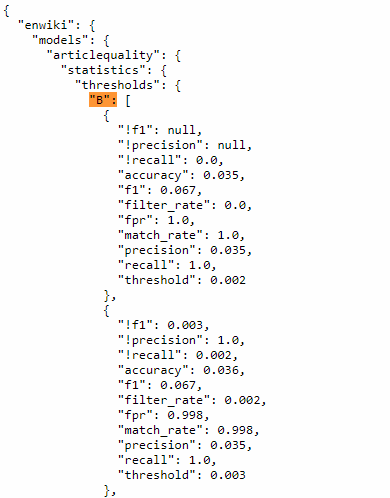
\includegraphics[scale=0.6]{resources/2/ORESarticlequalityThresholds}
\end{description}
\subsubsection{Different parameters}
Same as above.
\section{Clearing up confusion about parameters from before}
Paper page 15: ``when a \colorbox{cyan}{threshold} is set on 0.299 likelihood of damaging=true,
then you can expect to get a  \colorbox{orange}{recall} of 0.751,  \colorbox{lime}{precision}of 0.215, and a \colorbox{pink}{filter-rate} of 0.88''
\begin{itemize}
\item \colorbox{cyan}{Threshold} on 0.299 of damaging=true $\rightarrow$ if probability that an article is damaging $\geq 0.299$, then it is declared as damaging
\item  \colorbox{orange}{Recall}: 0.751 $\rightarrow$ given threshold catches 75.1\% of (most) damaging edits
\item  \colorbox{lime}{Precision}: 0.251 $\rightarrow$ approx. $\frac{1}{4}$ of edits, declared as damaging, actually are 
\item \colorbox{pink}{Filter-rate}: 0.88 $\rightarrow$ work of vandal-fighters reduced by 88\%
\end{itemize}
\section{Specifying parameters II}
\subsection{Querying formulas}
Paper:
\begin{itemize}
\item \url{https://ores.wikimedia.org/v3/scores/enwiki/?models=damaging&model_info=statistics.thresholds.true.'maximum filter_rate @ recall >= 0.75'} $\rightarrow$ write as ''\textbf{maximum filter\_rate @ recall $>=$ 0.75}''
\item \href{https://ores.wikimedia.org/v3/scores/enwiki/?models=damaging&model_info=statistics.thresholds.true.%27maximum%20recall%20@%20precision%20%3E=%200.9%27}{\textbf{maximum recall @ precision $>=$ 0.9}} produces:
\end{itemize}
\begin{description}
\item 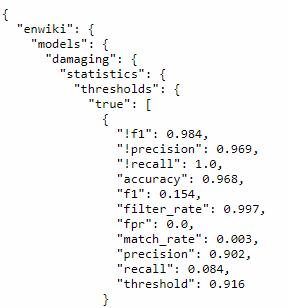
\includegraphics[scale=0.7]{resources/2/ORESmaxFilterAtRecall}
\end{description}
\begin{itemize}
\item \textbf{maximum} can be replaced with \textbf{minimum}
\item $>=$ can be replaced with $<=$
\item Both parameters can be replaced with any from the list above (except threshold ofc, which is not a parameter)
\end{itemize}
\newpage
\section*{Parameters to use in ORES' API queries}
Example format: \url{https://ores.wikimedia.org/v3/scores/enwiki/?models=damaging&model_info=statistics.thresholds.true.'maximum filter_rate @ recall >= 0.75'}
\begin{description}
\item (spaces: maximum\colorbox{red}{ }filter\_rate\colorbox{red}{ }@\colorbox{red}{ }recall\colorbox{red}{ }$>$=\colorbox{red}{ }0.75' or ``\%20'' in HTTP)
\end{description}
\begin{itemize}
\item !f1
\item !precision
\item !recall
\item accuracy
\item f1
\item filter\_rate
\item fpr
\item match\_rate
\item precision
\item recall
\end{itemize}
\end{document}
